\chapter{Custom code}
\label{chap:custom_code}

%\emph{creation of a new type of 2D code, based on previously seen concepts}
In this chapter, we will create a new type of 2D code, based on concepts discussed in this work: the Lycacode.

Some design choices have been made for ease of use and others for aesthetic purposes, each explained in their relevant section.

The basic format is in the form of a trefoil cross, the blazon of Saint-Maurice and of the Collège de l'Abbaye.

\begin{figure}[H]
  \centering
  
\includegraphics[width=0.4\textwidth]{images/lycacode_cross}
  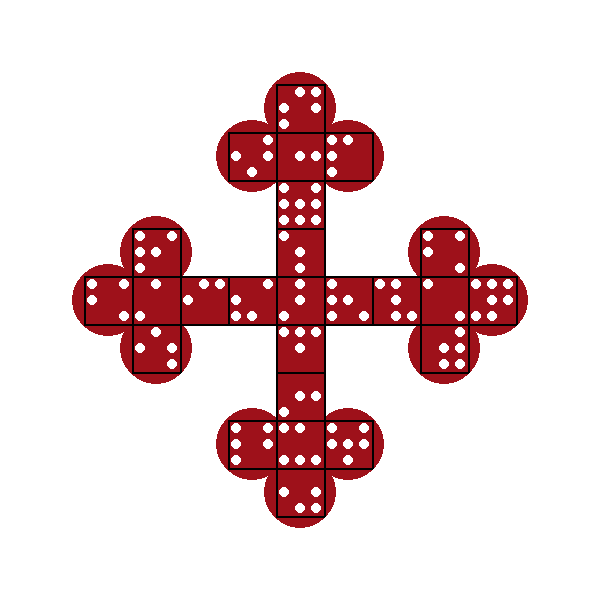
\includegraphics[width=0.4\textwidth]{images/lycacode_squares}
  \caption{Lycacode: trefoil cross and squares}
  \label{fig:lycacode_cross}
\end{figure}

%\begin{figure}[H]
%  \centering
%  
\includegraphics[width=0.5\textwidth]{images/lycacode_cross}
%  \caption{Custom code: trefoil cross}
%  \label{fig:lycacode_cross}
%\end{figure}

This cross is split into 25 squares which hold data. Each square is made of a 3x3 grid of dots and blanks, representing bits. The right of figure \ref{fig:lycacode_cross} shows how data (white dots) is put in the squares (highlighted in black)\footnote{the black squares are simply visual aids and are not part of the final code}. A dot represents a 1 while the absence of one is a 0.

The decision of using a grid-like pattern is convient for data placement as well as for reading the code.

The central square is reserved for the orientation pattern, as described in \autoref{ssec:lycacode_ex_layout}.
Additionally, the three top- and bottom-most dots are saved for the mask id (see \autoref{ssec:lycacode_ex_mask}).

\section{Encoding}
\label{sec:lycacode_encoding}

This code can work in one of four modes:
\begin{enumerate}
  \setcounter{enumi}{-1}
  \item Person
  \item Location
  \item Link
  \item Text
\end{enumerate}

\subsection{Person - mode 0}
\label{ssec:lycacode_mode0}

In mode 0, the code represents a person from the school. It can either be a student (type 0), a teacher (type 1) or someone else (type 2), such as the cleaning staff or caretaker. Table \ref{tab:lycacode_person} lists the different values encoded by each type and their corresponding bit size. Column "bit size" is the number of bits the value is encoded on. These have been chosen to use as few bits as possible to leave room for possible future additional data.

\def\arraystretch{1.5}
\begin{table}[H]
  \centering
  \begin{tabu}{|[2pt]l|l|c|[2pt]}
    \tabucline[2pt]{-}
    Type & Value & Bit size\\
    \tabucline[1pt]{-}
    \multirow{5}{*}{Student} & type & 2 \\
    \cline{2-3}
                             & id & 20 \\
    \cline{2-3}
                             & year & 3 \\
    \cline{2-3}
                             & class & 4 \\
    \cline{2-3}
                             & initials & 10 \\
    \tabucline[1pt]{-}
    \multirow{2}{*}{Teacher} & type & 2 \\
    \cline{2-3}
                             & id & 20 \\
    \tabucline[1pt]{-}
    \multirow{2}{*}{Other} & type & 2 \\
    \cline{2-3}
                             & id & 20 \\
    \tabucline[2pt]{-}
  \end{tabu}
  \caption{Lycacode: person mode - values}
  \label{tab:lycacode_person}
\end{table}
\def\arraystretch{1}

\textbf{For students}

\texttt{year} is the year number. DUBS is represented by the value 0.\\
\texttt{class} is the index of the class letter in the alphabet, starting from 0. For example, D is 3.\\
\texttt{initials} represent the initial of the firstname and that of the lastname, each as 5 bit numbers. The value of each letter is their index in the alphabet, starting from 0.

\paragraph{Example}

\begin{center}
  \begin{tabular}{c|c|c|c|c}
    type & id & year & class & initials \\
    \hline
    Student & 16048 & 5 & D & LH\\
  \end{tabular}

  Bits: 00 / 00 / 00000011111010110000 / 101 / 0011 / 01011 / 00111
\end{center}

\subsection{Location - mode 1}
\label{ssec:lycacode_mode1}

In mode 1, the code represents a location in the school. The section is encoded on 3 bits according to the following table:

\def\arraystretch{1.5}
\begin{table}[H]
  \centering
  \begin{tabu}{|[2pt]c|c|[2pt]}
    \tabucline[2pt]{-}
    Section & Value \\
    \tabucline[1pt]{-}
    A & 0 \\
    \hline
    B & 1 \\
    \hline
    C & 2 \\
    \hline
    D & 3 \\
    \hline
    Boarding school & 4 \\
    \hline
    "Bateau" & 5 \\
    \hline
    Sports alley & 6 \\
    \hline
    Football fields & 7 \\
    \tabucline[2pt]{-}
  \end{tabu}
  \caption{Lycacode: location mode - sections}
  \label{tab:lycacode_loc_sections}
\end{table}
\def\arraystretch{1}

Additionally the room number (or other id) is encoded on 9 bits.

\paragraph{Example}

\begin{center}
  \begin{tabular}{c|c}
    section & room \\
    \hline
    4 & 209 \\
  \end{tabular}

  Bits: 01 / 100 / 011010001
\end{center}

\subsection{Link - mode 2}
\label{ssec:lycacode_mode2}

In mode 2, the code represents a URL. The actual URLs are stored in a database and only the id is saved on the code as a 32 bit number. Scanners then fetch the URL info from the server's database.

\subsection{Text - mode 3}
\label{ssec:lycacode_mode3}

In mode 3, the code represents normal text. Text data is simply converted to UTF-8. The number of encoded characters is first encoded on 4 bits and added before text data. Due to its limited capacity, a Lycacode can only store up to 14 characters.

\paragraph{Example}

\begin{center}
  \begin{tabular}{c|c}
    length & text \\
    \hline
    4 & Lyca \\
  \end{tabular}

  Bits: 11 / 0100 / 01001100 / 01111001 / 01100011 / 01100001
\end{center}

\section{Error correction}
\label{sec:lycacode_err_corr}

It goes without saying that this code uses some kind of error correction. To keep it simple enough, Hamming(7, 4) codes have been chosen to fulfil this role. Encoded data is first padded to the maximum number of data bits $M$:

\[
  M = T * R
\]

where $T$ is the total number of bits which can be encoded on the cross and $R$ is the ratio of data bits over blocksize (here, $R = \frac{4}{7}$). $T$ can be calculated as follows:

\[
  T = \underbrace{3^2}_{\substack{\text{number of dots} \\ \text{in a square}}} * 24 - \underbrace{6}_{\text{mask id}}
\]

\section{Example}
\label{sec:lycacode_example}

Let's create a Lycacode to illustrate. We will make a student code using the values from the example in \autoref{ssec:lycacode_mode0}.

\subsection{Data encoding}
\label{ssec:lycacode_ex_encoding}

Table \ref{tab:lycacode_ex_values} lists all values to encode and their respective binary strings.

\def\arraystretch{1.5}
\begin{table}[H]
  \centering
  \begin{tabu}{|[2pt]l|c|l|[2pt]}
    \tabucline[2pt]{-}
    Property & Value & Binary\\
    \tabucline[1pt]{-}
    Mode & 0 & 00 \\
    \hline
    Type & 0 (=student) & 00 \\
    \hline
    Id & 16048 & 00000011111010110000 \\
    \hline
    Year & 5 & 101 \\
    \hline
    Class & 3 (=D) & 0011 \\
    \hline
    Initials & LH & 01011 00111 \\
    \hline
    \tabucline[2pt]{-}
  \end{tabu}
  \caption{Lycacode: example values}
  \label{tab:lycacode_ex_values}
\end{table}
\def\arraystretch{1}

The raw data bit string is thus:

\[
  \underbrace{00}_{\text{mode}} \underbrace{00}_{\text{type}} \underbrace{00000011111010110000}_{\text{id}} \underbrace{101}_{\text{year}} \underbrace{0011}_{\text{class}} \underbrace{0101100111}_{\text{initials}}
\]

We then need to pad it to fill the remaining free bits. First we pad with zeros to the nearest multiple of 4 (data bits per block).
Then we fill the rest with a pattern of consecutive binary numbers\footnote{the pattern is the series of natural numbers in binary starting from 0, e.g. 0, 1, 10, 11, 100, ...}, like this:

\[
  01101110010111011110001001101010111100110111101111...
\]
%We then pad it on the right with zeros to fill the remaining free bits M=124 (see section \ref{sec:lycacode_err_corr}) and construct the Hamming codes:
This pattern has the sole purpose of adding pseudo-random data so that there is data on the whole code. This is only an aesthetic choice.

\pagebreak

\subsection{Hamming codes}
\label{ssec:lycacode_ex_hamming}

Finally we construct the Hamming codes:

\def\arraystretch{1.5}
\begin{table}[H]
  \centering
  \resizebox{0.4\textwidth}{!}{
  \begin{tabu}{|[2pt]c|c|c|c|c|c|c|c|[2pt]}
    \tabucline[2pt]{-}
     & 1 & 2 & 3 & 4 & 5 & 6 & 7 \\
    \tabucline[1pt]{-}
    Group 1 & \_ & \_ & 0 & \_ & 0 & 0 & 0 \\
    \hline
    Group 2 & \_ & \_ & 0 & \_ & 0 & 0 & 0 \\
    \hline
    Group 3 & \_ & \_ & 0 & \_ & 0 & 1 & 1 \\
    \hline
    Group 4 & \_ & \_ & 1 & \_ & 1 & 1 & 0 \\
    \hline
    Group 5 & \_ & \_ & 1 & \_ & 0 & 1 & 1 \\
    \hline
    Group 6 & \_ & \_ & 0 & \_ & 0 & 0 & 0 \\
    \hline
    Group 7 & \_ & \_ & 1 & \_ & 0 & 1 & 0 \\
    \hline
    Group 8 & \_ & \_ & 0 & \_ & 1 & 1 & 0 \\
    \hline
    Group 9 & \_ & \_ & 1 & \_ & 0 & 1 & 1 \\
    \hline
    Group 10 & \_ & \_ & 0 & \_ & 0 & 1 & 1 \\
    \hline
    Group 11 & \_ & \_ & 1 & \_ & 0 & 0 & 0 \\
    \hline
    Group 12 & \_ & \_ & 0 & \_ & 1 & 1 & 0 \\
    \hline
    Group 13 & \_ & \_ & 1 & \_ & 1 & 1 & 0 \\
    \hline
    Group 14 & \_ & \_ & 0 & \_ & 1 & 0 & 1 \\
    \hline
    Group 15 & \_ & \_ & 1 & \_ & 1 & 0 & 1 \\
    \hline
    Group 16 & \_ & \_ & 1 & \_ & 1 & 1 & 0 \\
    \hline
    Group 17 & \_ & \_ & 0 & \_ & 0 & 1 & 0 \\
    \hline
    Group 18 & \_ & \_ & 0 & \_ & 1 & 1 & 0 \\
    \hline
    Group 19 & \_ & \_ & 1 & \_ & 0 & 1 & 0 \\
    \hline
    Group 20 & \_ & \_ & 1 & \_ & 1 & 1 & 1 \\
    \hline
    Group 21 & \_ & \_ & 0 & \_ & 0 & 1 & 1 \\
    \hline
    Group 22 & \_ & \_ & 0 & \_ & 1 & 1 & 1 \\
    \hline
    Group 23 & \_ & \_ & 1 & \_ & 0 & 1 & 1 \\
    \hline
    Group 24 & \_ & \_ & 1 & \_ & 1 & 1 & 0 \\
    \hline
    Group 25 & \_ & \_ & 0 & \_ & 0 & 0 & 1 \\
    \hline
    Group 26 & \_ & \_ & 0 & \_ & 0 & 0 & 1 \\
    \hline
    Group 27 & \_ & \_ & 1 & \_ & 0 & 0 & 1 \\
    \hline
    Group 28 & \_ & \_ & 0 & \_ & 1 & 0 & 0 \\
    \hline
    Group 29 & \_ & \_ & 1 & \_ & 1 & 1 & 0 \\
    \hline
    Group 30 & \_ & \_ & 1 & \_ & 0 & 0 & 1 \\
    \tabucline[2pt]{-}
  \end{tabu}}
  \resizebox{0.4\textwidth}{!}{
  \begin{tabu}{|[2pt]c|c|c|c|c|c|c|c|[2pt]}
    \tabucline[2pt]{-}
     & 1 & 2 & 3 & 4 & 5 & 6 & 7 \\
    \tabucline[1pt]{-}
    Group 1 & 0 & 0 & 0 & 0 & 0 & 0 & 0 \\
    \hline
    Group 2 & 0 & 0 & 0 & 0 & 0 & 0 & 0 \\
    \hline
    Group 3 & 1 & 0 & 0 & 0 & 0 & 1 & 1 \\
    \hline
    Group 4 & 0 & 0 & 1 & 0 & 1 & 1 & 0 \\
    \hline
    Group 5 & 0 & 1 & 1 & 0 & 0 & 1 & 1 \\
    \hline
    Group 6 & 0 & 0 & 0 & 0 & 0 & 0 & 0 \\
    \hline
    Group 7 & 1 & 0 & 1 & 1 & 0 & 1 & 0 \\
    \hline
    Group 8 & 1 & 1 & 0 & 0 & 1 & 1 & 0 \\
    \hline
    Group 9 & 0 & 1 & 1 & 0 & 0 & 1 & 1 \\
    \hline
    Group 10 & 1 & 0 & 0 & 0 & 0 & 1 & 1 \\
    \hline
    Group 11 & 1 & 1 & 1 & 0 & 0 & 0 & 0 \\
    \hline
    Group 12 & 1 & 1 & 0 & 0 & 1 & 1 & 0 \\
    \hline
    Group 13 & 0 & 0 & 1 & 0 & 1 & 1 & 0 \\
    \hline
    Group 14 & 0 & 1 & 0 & 0 & 1 & 0 & 1 \\
    \hline
    Group 15 & 1 & 0 & 1 & 0 & 1 & 0 & 1 \\
    \hline
    Group 16 & 0 & 0 & 1 & 0 & 1 & 1 & 0 \\
    \hline
    Group 17 & 0 & 1 & 0 & 1 & 0 & 1 & 0 \\
    \hline
    Group 18 & 1 & 1 & 0 & 0 & 1 & 1 & 0 \\
    \hline
    Group 19 & 1 & 0 & 1 & 1 & 0 & 1 & 0 \\
    \hline
    Group 20 & 1 & 1 & 1 & 1 & 1 & 1 & 1 \\
    \hline
    Group 21 & 1 & 0 & 0 & 0 & 0 & 1 & 1 \\
    \hline
    Group 22 & 0 & 0 & 0 & 1 & 1 & 1 & 1 \\
    \hline
    Group 23 & 0 & 1 & 1 & 0 & 0 & 1 & 1 \\
    \hline
    Group 24 & 0 & 0 & 1 & 0 & 1 & 1 & 0 \\
    \hline
    Group 25 & 1 & 1 & 0 & 1 & 0 & 0 & 1 \\
    \hline
    Group 26 & 1 & 1 & 0 & 1 & 0 & 0 & 1 \\
    \hline
    Group 27 & 0 & 0 & 1 & 1 & 0 & 0 & 1 \\
    \hline
    Group 28 & 1 & 0 & 0 & 1 & 1 & 0 & 0 \\
    \hline
    Group 29 & 0 & 0 & 1 & 0 & 1 & 1 & 0 \\
    \hline
    Group 30 & 0 & 0 & 1 & 1 & 0 & 0 & 1 \\
    \tabucline[2pt]{-}
  \end{tabu}}
  \caption{Lycacode: example hamming codes}
  \label{tab:lycacode_ex_hamming}
\end{table}
\def\arraystretch{1}

\subsection{Laying out data}
\label{ssec:lycacode_ex_layout}

The matrix layout is shown in figure \ref{fig:lycacode_layout}. Notice the center square; it is used for rotation and mirror image detection.
The middle pattern has to be asymmetrical both in reflection and rotation. Here, the top dot helps determine rotation, while the left one is used to check whether the code is mirrored or not.
The central dot indicates that this is a Lycacode. Indeed, another type of code, Mini Lycacodes, has been created. Those don't have this dot, signaling that they are Mini Lycacodes.\footnote{Mini Lycacodes are not described here but are implemented in Python in the files \texttt{lycacode\_gen\_mini.py} and \texttt{lycacode\_scanner\_mini.py}}

The top and bottom gray areas are reserved for the mask id as explained later.
Also note that white means 1 and black 0.

Starting from the top left going in reading direction, the bits are layed out in the free areas. As for QR-Codes, the first bit of each group is first layed, then the second, the third and so on. Figure \ref{fig:lycacode_ex_data_layout} shows the result of this step. The interleaving process allow a division of data in such a way that if a portion of the code is unreadable, the errors are distributed accross multiple data blocks, increasing the chance of recovery (since each block can only correct one bit).

\begin{figure}[H]
  \centering
  \begin{subfigure}{0.4\textwidth}
    \centering
    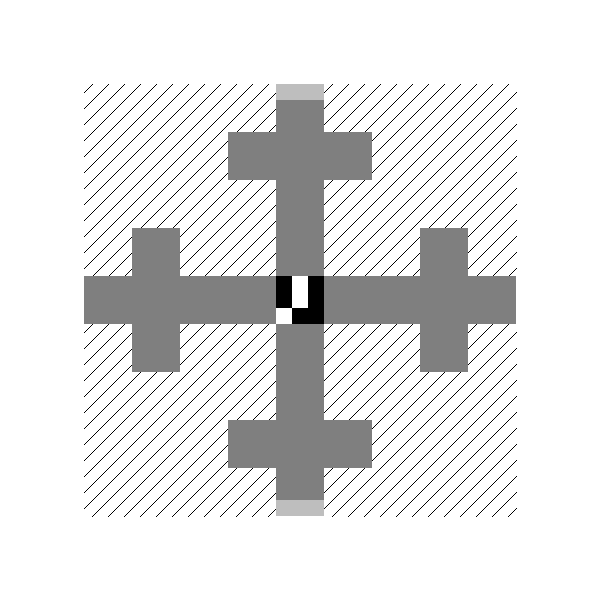
\includegraphics[width=\textwidth]{images/lycacode_layout}
    \caption{Empty}
    \label{fig:lycacode_layout}
  \end{subfigure}
  \begin{subfigure}{0.4\textwidth}
    \centering
    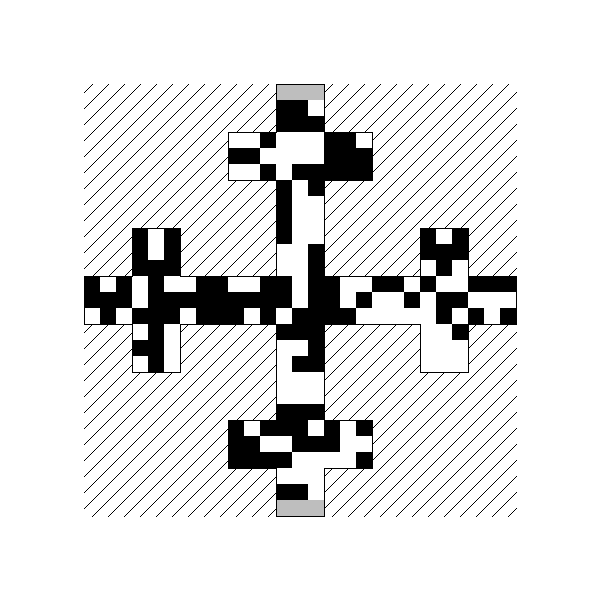
\includegraphics[width=\textwidth]{images/lycacode_data_layout}
    \caption{With data}
    \label{fig:lycacode_ex_data_layout}
  \end{subfigure}
  \caption{Lycacode layout}
\end{figure}

\subsection{Mask}
\label{ssec:lycacode_ex_mask}

As a last step, a mask is applied. The 8 masks are described in figure \ref{fig:lycacode_masks}. The best fitting one is selected based upon similar criteria as for QR-Codes\footnote{the exact criteria are defined in the python script \texttt{lycacode\_gen.py}}. Once applied to the data bits, the mask's id is encoded on the 3 reserved bits at the top and bottom of the code.

The purpose of masking in this context is purely aesthetical. It is a mean to avoid unpleasant visual patterns in the final code.

\begin{figure}[H]
  \centering
  \begin{subfigure}{0.4\textwidth}
    \centering
    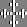
\includegraphics[width=0.4\textwidth]{images/lycacode_mask_0}
    \caption{x mod 3 = 0}
    \label{fig:lycacode_mask_0}
  \end{subfigure}
  \begin{subfigure}{0.4\textwidth}
    \centering
    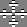
\includegraphics[width=0.4\textwidth]{images/lycacode_mask_1}
    \caption{y mod 3 = 0}
    \label{fig:lycacode_mask_1}
  \end{subfigure}
  \begin{subfigure}{0.4\textwidth}
    \centering
    
\includegraphics[width=0.4\textwidth]{images/lycacode_mask_2}
    \caption{(x+y) mod 3 = 0}
    \label{fig:lycacode_mask_2}
  \end{subfigure}
  \begin{subfigure}{0.4\textwidth}
    \centering
    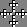
\includegraphics[width=0.4\textwidth]{images/lycacode_mask_3}
    \caption{(x mod 3)*(y mod 3) = 0}
    \label{fig:lycacode_mask_3}
  \end{subfigure}
  \begin{subfigure}{0.4\textwidth}
    \centering
    
\includegraphics[width=0.4\textwidth]{images/lycacode_mask_4}
    \caption{(y//3+x//3) mod 2 = 0}
    \label{fig:lycacode_mask_4}
  \end{subfigure}
  \begin{subfigure}{0.4\textwidth}
    \centering
    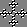
\includegraphics[width=0.4\textwidth]{images/lycacode_mask_5}
    \caption{[(y mod 3)-1]*[(x mod 3)-(y mod 3)-2]*[(y mod 3)-(x mod 3)-2] = 0}
    \label{fig:lycacode_mask_5}
  \end{subfigure}
  \begin{subfigure}{0.4\textwidth}
    \centering
    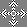
\includegraphics[width=0.4\textwidth]{images/lycacode_mask_6}
    \caption{(|13-x|+|13-y|) mod 3 = 1}
    \label{fig:lycacode_mask_6}
  \end{subfigure}
  \begin{subfigure}{0.4\textwidth}
    \centering
    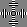
\includegraphics[width=0.4\textwidth]{images/lycacode_mask_7}
    \caption{[1-(x mod 2) + max(0, |13-y|-|13-x|)] * [1-(y mod 2) + max(0,|13-x|-|13-y|)] = 0}
    \label{fig:lycacode_mask_7}
  \end{subfigure}
  \caption{Lycacode masks}
  \label{fig:lycacode_masks}
\end{figure}

Note: "//" is integer division

For our example, the best mask is mask 3. The final binary matrix is shown in figure \ref{fig:lycacode_ex_final_mat}.

\begin{figure}[H]
  \centering
  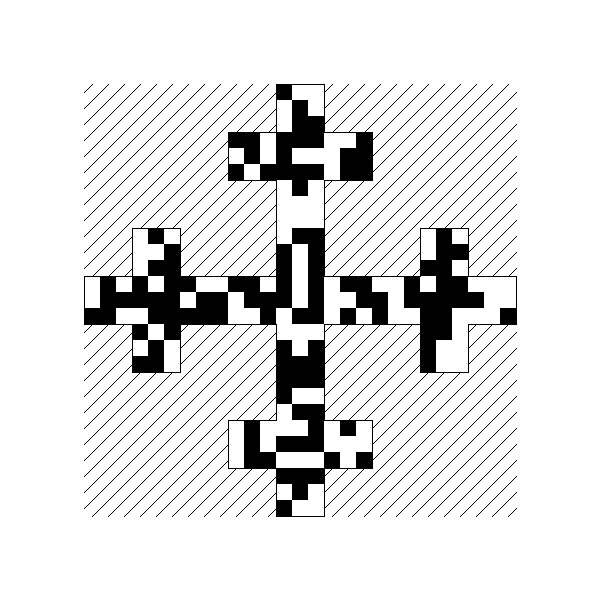
\includegraphics[width=0.5\textwidth]{images/lycacode_ex_final_mat}
  \caption{Lycacode example: masked matrix}
  \label{fig:lycacode_ex_final_mat}
\end{figure}

Finally, the matrix is converted to white dots (for 1s) on the red trefoil cross shown in figure \ref{fig:lycacode_cross}, giving the final code in figure \ref{fig:lycacode_ex_final}.

\begin{figure}[H]
  \centering
  
\includegraphics[width=0.5\textwidth]{images/lycacode_ex_final}
  \caption{Lycacode example: final code}
  \label{fig:lycacode_ex_final}
\end{figure}

The external square is used to detect the code and to correct perspective.
Its position and dimensions, which have been chosen quite arbitrarily, are visualized on figure \ref{fig:lycacode_frame}. In fact, only the position and size of the inner border is relevant in the decoding process.

\begin{figure}[H]
  \centering
  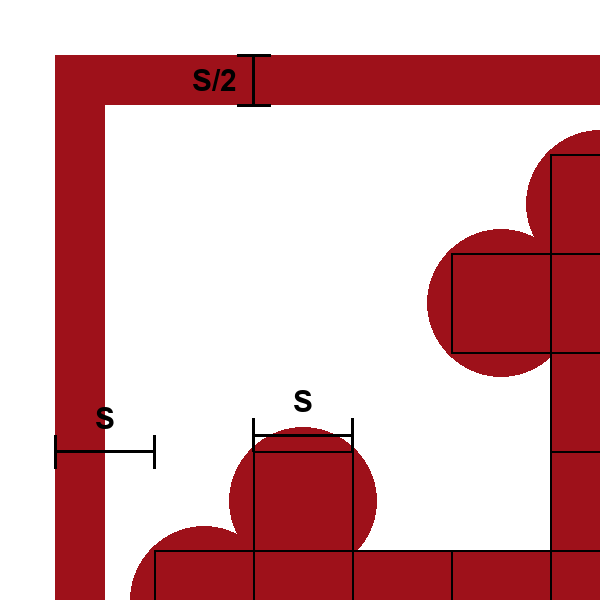
\includegraphics[width=0.5\textwidth]{images/lycacode_frame}
  \caption{Lycacode frame dimensions}
  \label{fig:lycacode_frame}
\end{figure}
